\documentclass[a4paper, 12pt, oneside, toc=listofnumbered, bibliography=totoc]{scrbook}
\usepackage[hyphens,spaces,obeyspaces]{url}
\usepackage[sorting = none, backend=bibtex]{biblatex}
\usepackage[german]{babel}
\usepackage[T1]{fontenc}
\usepackage[utf8]{inputenc}
\usepackage[hidelinks]{hyperref}
\usepackage{graphicx}
\usepackage{subcaption}
\usepackage{epstopdf}
\usepackage{lmodern}
\usepackage{float}
\usepackage{acronym}
\usepackage{booktabs}
\usepackage{caption}
\usepackage{csquotes}
\usepackage{enumitem}
\usepackage{fancyhdr}
\usepackage{url}
\usepackage{listings}
\usepackage[table]{xcolor}
\usepackage{wrapfig}
\usepackage{forest}
\usepackage{tabularx}
\usepackage{colortbl}
\usepackage{booktabs}
\usepackage[onehalfspacing]{setspace}
\usepackage{amsmath}
\usepackage{threeparttable}
\usepackage[german]{cleveref}
\usepackage{parskip}

\renewcommand*{\headfont}{\normalfont}
\renewcommand*{\multicitedelim}{\addsemicolon\space}
\renewcommand*{\headrulewidth}{0pt}
\renewcommand*{\arraystretch}{1.5}
\setlength{\parskip}{1.5ex}
\makeatletter
% define new boolean conditional switch for whether
% the abstract is being typeset
\newif\ifabstract
% redefine `\chapter` so it only starts a new page if not typesetting
% the abstract; sets abstract conditional to false after doing so
\renewcommand\chapter{\ifabstract\relax\else%
	\if@openright\cleardoublepage\else\clearpage\fi%
	\fi
	\abstractfalse%
	\thispagestyle{plain}%
	\global\@topnum\z@
	\@afterindentfalse
	\secdef\@chapter\@schapter}

% command for putting the title and name above the abstract; switches
% abstact boolean to true for next `\chapter*` command...
\newcommand{\conclusion}{
	\if@openright\cleardoublepage\else\clearpage\fi
		\begin{center}
			\textbf{\larger{Summary}}\par
			\emph{Hier kommt nach der Fertigstellung der Arbeit noch eine Zusammenfassung der Arbeit mit ein oder mehreren Sätzen hin. Hier kommt nach der Fertigstellung der Arbeit noch eine Zusammenfassung der Arbeit mit ein oder mehreren Sätzen hin. Hier kommt nach der Fertigstellung der Arbeit noch eine Zusammenfassung der Arbeit mit ein oder mehreren Sätzen hin2. }\par
		\end{center}

	\abstracttrue}
\makeatother
\lstset
{
         basicstyle=\footnotesize\ttfamily,
         numbers=left,               	% Ort der Zeilennummern
         numberstyle=\tiny,          	% Stil der Zeilennummern
%         stepnumber=2,               	% Abstand zwischen den Zeilennummern
         numbersep=5pt,              	% Abstand der Nummern zum Text
         tabsize=2,                  	% Groesse von Tabs
         extendedchars=true,
         breaklines=true,            	% Zeilen werden Umgebrochen
         keywordstyle=\color{red},
            frame=b,
 %        keywordstyle=[1]\textbf,    	% Stil der Keywords
 %        keywordstyle=[2]\textbf,
 %        keywordstyle=[3]\textbf,
 %        keywordstyle=[4]\textbf, \sqrt{\sqrt{}}
         stringstyle=\color{white}\ttfamily,
         showspaces=false,
         showtabs=false,
         xleftmargin=27pt,
         framexleftmargin=27pt,
         framexrightmargin=5pt,
         framexbottommargin=4pt,
%         backgroundcolor=\color{lightgray},
         showstringspaces=false      	% Leerzeichen in Strings anzeigen ?
}
\addbibresource{Bachelorarbeit.bib}
\setuptoc{toc}{numbered}

\begin{document}
	\frontmatter
	\def\doctype{Bachelorarbeit}
\def\title{Vorgehensweise zur Implementierung der VDMA Spezifikation „OPC UA for Machinery (OPC 40 001)“ in Maschinen und IT-Systemen erarbeiten}
\def\author{Rico Kursidem}
\def\supervisor{Dipl. Ing (FH) Michalowski}
\def\supervisortwo{Prof. Dr. Mielebacher}

\begin{titlepage}

\vspace{10mm}

\begin{center}
	
	\vspace{5mm}
	\huge \title
	
	\vspace{34pt}
	\large \doctype
		
	\vspace{30pt}	
	\small Angewandte Informatik \\
	\large Duale Hochschule Baden-Württemberg Mosbach \\
	\small Studienpartner \\
	\large AZO GmbH \& Co. KG \\
    \vspace{35pt}
    
    
\includegraphics[height=2.5cm]{prefix/image/logo-dhbw.eps}
    
\includegraphics[height=2.5cm]{prefix/image/logo-azo.png}
	
	\vspace{40pt}	
	\small von \\
	\large \author \\
	\small betreut von \\
	\large \supervisor \\
	\small und \\
	\large \supervisortwo

\end{center}

\vspace{75pt}


\vspace{49.7pt}

\fancypagestyle{empty}{
  \fancyhf{}
  \fancyfoot[C]{\today}
}

\end{titlepage}
	\chapter*{Abkürzungsverzeichnis} 
\begin{acronym}
	%A
	\acro{API}{Advanced Programming Interface}
	%B
	%C
	\acro{COM}{Component Object Model}
	%D
	\acro{DCOM}{Distrebuted Component Object Model}
	%E
	\acro{ERP}{Enterprse Recource Planning}
	%F
	%G
	%H
	\acro{HMI}{Human Maschine Interface}
	%I
	\acro{IoT}{Internet of Things}
	%J
	%K
	%L
	%M
	\acro{M2M}{Maschine-zu-Maschine}
	\acro{MES}{Manufacturing Execution System}
	\acro{MQTT}{Message Queuing Telemetry Transport}
	%N
	%O
	\acro{OPC UA}{Open Platform Communications Unified Architecture}
	%P
	%Q
	%R
	%S
	\acro{SOA}{Service orientierte Architektur}
	%T
	\acro{TCP/IP}{Transmission Control Protocol/Internet Protocol}
	%U
	\acro{UMATI}{Universal machien technology interface}
	%V
	\acro{VDMA}{Verband Deutscher Maschinen- und Anlagenbau}
	\acro{VDW}{Verein Deutscher Werkzeugmaschinenfabriken e.V. }
	%W
	%X
	%Y
	%Z
\end{acronym}
	\tableofcontents
	\listoffigures
	%\listoftables
	%\lstlistoflistings
	\nocite{*}

	
	
	\chapter*{Abstract}
	
	\section*{Deutsch}
	
	\section*{English}
	
	
	\mainmatter
	\pagebreak
%	\conclusionpng
	\chapter{Einführung}\label{ch:Einführung}
	% (4 Seiten)
	
	Die moderne Welt wird zunehmend vernetzter. Unternehmen weiten ihre Wertschöpfungsketten global aus und erzeugen so ein weltweites Abhängigkeitsnetz. Unternehmen erweitern Ihren Kundenmarkt auf die gesamte Welt und beziehen von überall Zulieferungen. In der Industrie ist es dabei besonders wichtig, dass alle Teilnehmer an Wertschöpfungsketten, Arbeitsgruppen und Verträgen dasselbe Verständnis von Daten haben. Um ein weltweit, einheitliches und unmissverständliches Kommunikationssystem zu ermöglichen, werden Standards verwendet. In Zeiten der Industrie 4.0 nehmen Standardisierungen einen noch wichtigeren Platz ein als zuvor. Da Anlagen immer mehr aus Maschinen verschiedenster Hersteller zusammengesetzt sind, ist ein gemeinsamer übergreifender Kommunikationsstandard besonders wichtig, um eine fehlerfreie, effiziente und wirtschaftliche Produktion zu ermöglichen.
	
	Standardisierung wird verwendet, um effizienteren Austausch und effektivere Prozesse durchzuführen. Ein sehr altes Beispiel sind Sprachen. Eine Menge an Regeln, welche zur Kommunikation genutzt werden, auf die sich alle Teilnehmenden geeinigt haben. In dieser Arbeit soll es um die Standardisierung im Bereich der \ac{M2M} Kommunikation gehen. Durch die Herausforderungen von Industrie 4.0 kann ein guter Standard die Integration mehrerer Systeme vereinfachen und Kosten sparen.
	
	In der M2M Kommunikation existieren bereits Standards, die schon vor Industrie 4.0 entworfen wurden. Dazu gehört \ac{OPC UA}. \ac{Umati} baut auf diesem Standard auf und definiert weitere Aspekte wie beispielsweise eine Plug \& Play Umgebung. Das Ziel von \ac{Umati} ist es, die zahlreichen Implementationen von OPC UA Schnittstellen zu standardisieren und zusammenzufassen, um so für Produzenten von Anlagen und Software einen gemeinsamen Standard zu finden. Das Ziel dieser Arbeit ist \ac{Umati} zu analysieren, die Implementation dieses Standards zu erforschen und ein Proof-of-Concept zu entwickeln, der die Fähigkeiten dieser Schnittstelle demonstriert.
	
	\section{Problemstellung und Ziel}
	
	% (1-2 Seiten)
	
	 Durch die zunehmende Automatisierung der Produktion und Fertigung stehen viele Produzenten vor der Aufgabe, zahlreiche Maschinen verschiedenster Hersteller in ihren Fertigungsprozess zu integrieren. Viele dieser Maschinen nutzen verschiedene Kommunikationsprotokolle, Datenformate und Schnittstellen, welche die Integration dieser diversen Systeme erschwert. Durch eine komplizierte Integration kann Vendor Lock-in entstehen. Dieses Konzept beschreibt die Bindung eines Kunden an einen Anbieter, da dieser eine Technologie oder Kommunikationsstrategie integriert, die andere Hersteller nicht oder nur extrem schwer integrieren können. Dies führt zu weniger Flexibilität und Kontrolle für den Kunden über das Projekt und steigert dessen Kosten. Um dieses Problem zu lösen, müssen sich die Produzenten zu einem Standard zusammenfinden und die Interoperabilität ihrer Systeme zu gewährleisten. \cite{mielebacher_verteilte_2021}
	 
	 Für AZO als Anlagenproduzent ist es von großem Interesse, mit Anlagen und Maschinen anderer Hersteller kommunizieren zu können und dabei die Integration einfach zu realisieren. Für Entwickler von \ac(MES) bedeutet die Standardisierung von Kommunikationsprotokollen eine schnellere und einfachere Entwicklung, was zu niedrigeren Entwicklungskosten führt und die Robustheit der Systeme erhöht. AZO nimmt an der Entwicklung von \ac{Umati} teil, um diese Standardisierung zu erreichen. Dieser Standard möchte die Schnittstellen für die Kommunikation zwischen Maschinen und mit der darüber liegenden Datenverarbeitung definieren und basiert auf dem offenen Standard \ac{OPC UA}.
	 
	 Das Ziel dieser Arbeit ist es, \ac{Umati} in einem Testumfeld anhand eines Proof-of-Conzept aufzubauen. Um dies zu erreichen, soll zunächst eine Marktanalyse durchgeführt werden, um mögliche Lösungen zum Versenden und Empfangen von Daten zwischen Maschine und \ac(MES) zu finden. Diese sollen anhand von selbst entwickelten Kriterien abgewogen und bewertet werden. Die vielversprechendsten Umsetzungen sollen in einem Testsystem implementiert werden und für zukünftige Demonstrationen auf Messen für AZO zur Verfügung gestellt werden.
	 
	 Dabei sollen zwei Systeme entstehen. Der VDMA bietet ein Web-Dashboard unter umati.app an, auf dem Zahlreiche Hersteller ihre Maschinen bereits Anbinden. Hier soll eine Simulierte Maschine von AZO ebenfalls dargestellt werden. Außerdem soll eine Interne Demonstration aufgebaut werden, die eine Umatifähige Maschine in die bestehende Infrastruktur Integriert und die Informationen Visualisieren kann.
	
	\section{Unternehmen}
	
	 Diese Arbeit wird mit dem Dualen Partner \textit{AZO Gmbh \& Co. KG} durchgeführt. AZO bietet maßgeschneiderte Lösungen für die automatisierte Förderung, Lagerung und Dosierung von Rohstoffen weltweit an. Dabei werden Anlagen für die Bereiche der Chemie-, Nahrungsmittel-, Pharma-, Kosmetik und Kunststoffindustrie gefertigt. Diese Projekte umfassen die Planung, Fertigung und Montage sowie die Automatisierung der Anlagen.
	 
	 AZO entwickelt ein eigenes MES-System ACAS, welches die Kommunikation zwischen Anlagen von AZO, aber auch Anlagen von anderen Herstellern, mit den Kunden vereinheitlichen und verbessern soll. Dabei soll ein umfassendes System entstehen, welches Steuerung, Visualisierung und Überwachung der Produktion übernehmen und in einer zentralen Software bündeln soll.
	 
	 ACAS entsteht in der Entwicklungsabteilung, welche ebenfalls an dieser Arbeit beteiligt ist. Sie fokussiert sich auf die Automatisierung von AZO Anlagen im Bereich von SPS, Steuerungen bis zur Datenverarbeitung und Erhebung auf abstrahierter Ebene. 
	
	%TODO: Was stellt mir AZO zur verfügung - System, Server, ...
	
	\section{Forschungsfragen}
	
	Die Standardisierung der Integration von verschiedensten Maschinen ist nötig und kann zu verstärkten Effizienzsteigerungen und Aufwandsersparnis führen. Für Anlagenbauer verspricht die Nutzung von \ac{Umati}, diese Integration in einen schnellen und effizienten Prozess zu wandeln. Um das Potenzial von \ac{Umati} zu evaluieren, wurden folgende Schwerpunkte betrachtet:
	
	\begin{itemize}
		\item \textbf{Q1}: Welche Herausforderungen ergeben sich bei der Umsetzung von \ac{Umati}?
		\item \textbf{Q2}: Welche Lösungen zur Umsetzung von \ac{Umati} sind am Wirtschaftlichsten?
		\item \textbf{Q3}: Wie kann die Datenkommunikation zwischen Anlage und Visualisierungplattform bestmöglich implementiert werden?
	\end{itemize}
	
	\section{Aufbau der Arbeit}
	
	Zu Beginn der Arbeit werden alle Grundlegenden Technologien und Themenbereiche beschrieben, die zum Verständnis benötigt werden (Kapitel \ref{ch:Grundlagen}). Daraufhin werden die Methodiken beschrieben, mit denen die Informationen für diese Arbeit erhoben wurden (Kapitel \ref{ch:Methodiken}). Im Hauptteil der Arbeit (Kapitel \ref{ch:Ergebnisse}) werden die Vorbereitenden Schritte für die Projekte sowie deren Durchführung behandelt. Die Implementation der Programme wird in Kapitel \ref{ch:Implementierung} in zwei Teilen behandelt, wobei die Implementation des Firmeninternen Prototyps aus Kapitel \ref{ch:Implementierung-Intern} auf die Ergebnisse aus Kapitel \ref{ch:Implementierung-Web} stützt. Die Arbeit schließt mit einer Diskussion der gefundenen Ergebnisse und einem Fazit (Kapitel \ref{ch:Diskussion_Fazit}).
	
	% TODO: Messematerial wenn in kapitel behandelt noch anhängen
	% TODO: Ganz am Schluss nochmal lesen
	
\chapter{Grundlagen}\label{ch:Grundlagen}
	% (16 Seiten)
	
	% Stand der Technik
	
	
	\section{OPC UA}
	
	%Einführung
	\ac{OPC UA} ist ein unternehmensunabhängiger, offener Standard zur Kommunikation von Informationen und Daten zwischen Maschinen im industriellen Umfeld. Das Protokoll wurde 2008 von der OPC Foundation veröffentlicht und nimmt sich zur Aufgabe, die Interoperabilität von Systemen zu fördern. Es verwendet eine \ac{SOA} und kann auf verschiedensten Betriebssystemen verwendet werden. OPC UA ist sehr gut skalierbar und kann deshalb als Kommunikationsprotokoll bei kleinen \ac{IoT} Systemen als auch bei komplexen Cloud-Systemen zur Anwendung kommen. 
	 
	 %Server-Client Modell
	OPC UA baut auf einem Server-Client-Modell auf, wobei der Client die Anfragen an den Server senden muss. Der Client fragt den Server nach Daten und analysiert diese während der Server die Daten der dahinterliegenden Anlagen in übertragbare Strukturen bringt und sie zur Verfügung stellt. Da der jeder Client an mehreren Servern Daten erheben kann, wird das System gut skalier- und erweiterbar.
	
	%Interoperabilität
	Das Ziel von OPC UA und auch im weitergetragenen Sinne von \ac{Umati} ist das Erreichen von Interoperabilität von Maschinen im industriellen Bereich. Interoperabilität beschreibt die Standardisierung von Kommunikation zwischen Systemen. Allgemein kann diese in 4 Stufen eingeteilt werden, wobei jede Ebene auf die darunterliegende aufbaut. Im Schaubild \ref{fig:Interoperabilität} sind die vier Ebenen strukturelle, syntaktische, semantische und organisatorische Interoperabilität abgebildet.
	 
	 \begin{figure}[H]
	 	\centering
	 	\includegraphics[width=0.9\textwidth]{res/diagramms/Interoperabilität.pdf}
	 	\caption{Die vier Ebenen der Interoperabilität}
	 	\label{fig:Interoperabilität}
	 \end{figure}
	 
	 %Ebene 1
	 Die strukturelle Interoperabilität beschreibt Verbindungen zwischen den Systemen, weshalb sie auch oft als Konnektivität bezeichnet wird. Der Datenaustausch kann nur erfolgen, wenn die beteiligten Systeme miteinander verbunden sind und ein geeignete Schnittstelle implementieren. Diese Verbundenheit kann über ein Netzwerk mit TCP/IP oder HTTP erreicht werden oder kann ein Übertragungsmedium wie USB festlegen. \cite{mielebacher_verteilte_2021}
	 
	 %Ebene 2
	 Sind Systeme syntaktisch interoperabel, nutzen und verstehen sie die Struktur der Daten. Hierfür können festgelegte Standards wie XML oder Json verwendet werden. \cite{mielebacher_verteilte_2021-1}
	 
	 %Ebene 3
	 Die semantische Interoperabilität beschreibt das vereinheitlichte Verständnis der Daten. Kommunizieren zwei Systeme miteinander, so müssen Sie unter denselben Werten auch dasselbe verstehen. Ein Beispiel für einen Standard, der semantische Interoperabilität umsetzt, ist der "International Classification of Diseases". Bei diesem geht es um die Kommunikation von Krankheiten zwischen Ärzten und wurde von der WHO eingeführt. Jede Krankheit hat einen festgelegten Code, wodurch eine eindeutige Kommunikation gewährleistet ist. \cite{mielebacher_verteilte_2021-1}
	 
	 %Was legt OPC UA fest
	 OPC UA legt anhand des Information-Models die Syntax der Daten fest, wodurch die syntaktische Interoperabilität gewährleistet ist. Die semantische Interoperabilität wird anhand der Companion Standards festgelegt, welche auf den OPC UA Standard aufgesetzt werden. Diese beschreiben Technologie-spezifische Informationsmodelle welche von verschiedensten Arbeitsgruppen erstellt werden. Es gibt unterschiedliche Companion Spezifikationen für unterschiedliche Anwendungsgebiete von OPC UA, beispielsweise für bestimmte Maschinengruppen oder Branchen. Sie legen jedoch immer fest, wie bestimmte Daten verstanden werden müssen. %TODO Quelle -> OPC Foundation?
	 
	 %OPC Classics
	 OPC UA entstand aus dem zuvor entwickelten Standard OPC Classics. Der alte Standard setzte die Kommunikation im Bereich der Automatisierung bereits sehr gut um. Der Nachteil an Classics war jedoch die fehlende Plattformunabhängigkeit. OPC UA unterstützt heute jegliche Betriebssysteme für Clients als auch für die Server, während der Vorgänger auf einem Windowssystem betreiben werden musste. Auch die Kommunikation war auf die von Microsoft entwickelte Technologien \ac{COM} und \ac{DCOM} ausgelegt. Durch die Ablösung dieses Standards durch OPC UA wird über TCP/IP und SOAP kommuniziert, welche beide Plattformunabhängig sind und somit kann OPC UA auch auf anderen Plattformen wie Linux, Mac und Android ohne Probleme angewandt werden. \cite{mielebacher_verteilte_2021-1}
	
		\subsection{Struktur}
		
		OPC UA ist eine Sammlung von Standards, welche in unterschiedlichen Spezifikationen definiert sind. Diese gliedern sich in eine hierarchische Struktur, welche dann bei der Implementierung aufeinander aufbauen. In Abbildung \ref{fig:OPCUA_Framework} ist die Struktur des UA Framework abgebildet. Im unteren Teil und somit der Grundbaustein dies Modells stehen Spezifikationen zum Transport und der Service Discovery. Diese beschreiben über welche Medien Daten transportiert wird und wie erkannt werden kann, welche Services existieren, die den OPC UA Standard implementieren. \cite{mahnke_opc_2009, rinke_was_2022}
		
		Zur Infrastruktur, welche im Allgemeinen die Konnektivität gewährleistet, ist auch die Spezifikation für den Datenzugang (Information Access) definiert. Außerdem werden auch weitere Standards beschrieben, um die Sicherheit und Robustheit des Systems zu gewährleisten.
		
		Auf den Standards der Infrastruktur bauen die Spezifikationen der Informationsmodelle auf. Diese bestehen aus den offiziellen OPC UA Spezifikationen und den darauf aufbauenden Companion und Vendor Informationsmodellen. \cite{mahnke_opc_2009}
		
		Die offiziellen Standards befassen sich mit dem allgemeinen Austausch von Daten. Hierzu gehören der Austausch von Echtzeitdaten (DA), historischen Daten (HA) und Alarmen (AC). Neben diesen Hauptfaktoren werden auch andere Standards festgelegt, die das offizielle OPC UA Information Modell bilden. \cite{mahnke_opc_2009, rinke_was_2022}
		
		%Companion Spezifikationen
		Auf dem OPC UA Standard setzen die Industriestandardinformation Modelle auf. Diese sind von mehreren Teilhabern entwickelte Standards, die beispielsweise innerhalb einer bestimmten Branche oder Industrie-Gruppen verwendet werden. Diese Standards stehen in den Companion Spezifikationen. Beispielsweise gibt es einzelnen Spezifikationen für AutoID Systeme oder Spritzgussmaschinen, die Abwandlungen und Spezialisierungen haben, die auf ihren Bereich angepasst sind. \cite{mahnke_opc_2009, rinke_was_2022}
		
		%Vendor Spezifikationen
		Auf der obersten Ebene des Schaubilds in Abbildung \ref{fig:OPCUA_Framework} sind die Vendor Informationsmodelle dargestellt. Diese sind weitere Standards, die die Companion Standards erweitern und innerhalb einer Maschinenumgebung eines Erstellers umgesetzt werden. In diesen Standards sind Veränderungen individueller Hersteller definiert, damit eine weitere Spezialisierung über die Companion Spezifikationen hinaus stattfinden kann. \cite{mahnke_opc_2009, rinke_was_2022}
		
		
		\begin{figure}[H]
			\centering
			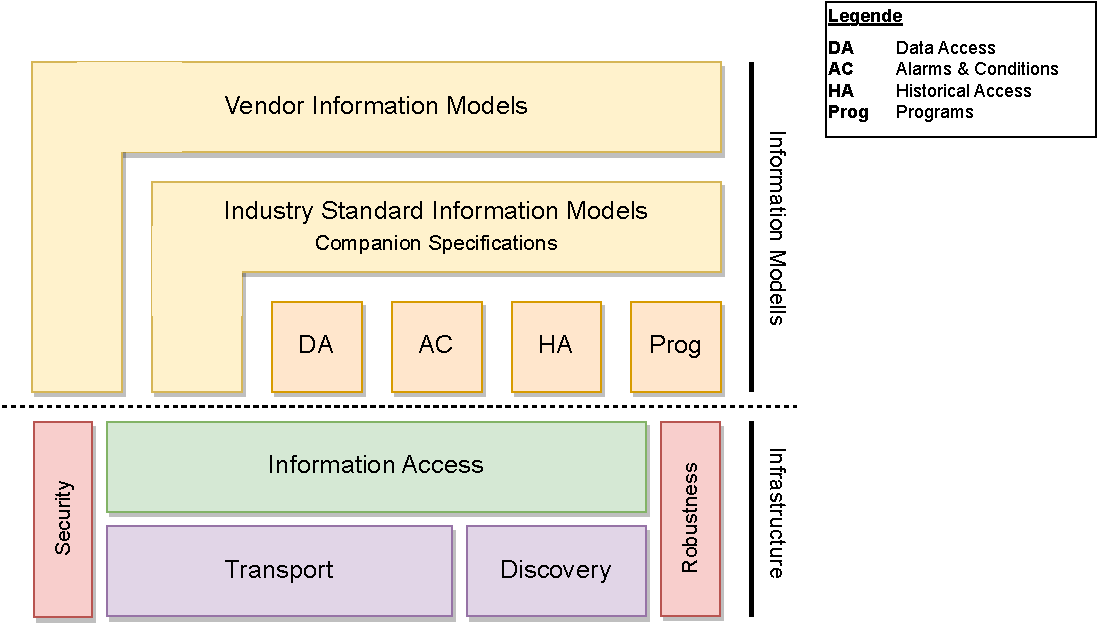
\includegraphics[width=0.9\textwidth]{res/diagramms/companionSpezifikations.pdf}
			\caption{Aufbau des OPC UA Standards, \\ Angelehnt an: Abbildung 1.7 in \cite{mahnke_opc_2009}} %TODO anständig machen
			\label{fig:OPCUA_Framework}
		\end{figure}
	
		\subsection{Kommunikationsaufbau} 
		
		%Client/Server/Field
		OPC UA besteht aus drei Komponenten, deren Zusammenwirkung in Abbildung \ref{fig:OPCUA_Structure} abgebildet ist. Mehrere Field Connections, die die Sensorik oder Maschinen darstellen, mit welchen kommuniziert werden soll. Die Daten sollen zu den OPC UA Clients geleitet werden. Dies können \ac{HMI} oder MES-Systeme sein, die die Daten der Maschinen auswerten oder Steuerungsbefehle absenden möchten. OPC UA standardisiert diese Kommunikation über den OPC UA Server. Dieser setzt den OPC UA Standard um und stellt das notwendige \ac{API} für die Datenabfrage aus der Sicht der Clients zur Verfügung. \cite{rinke_was_2022}
		
		%Integriert oder nicht
		Der OPC UA Server implementiert die proprietären Kommunikationsprotokolle, die vom Maschinenhersteller entwickelt wurden, um mit den Anlagen und den Field Conections zu kommunizieren. Je nach Art der Daten, die die Maschine weiter gibt, werden die Daten auf dem OPC UA Server abgespeichert oder an den Client weiter gegeben. Ein OPC UA Server kann in zwei Formen entstehen. Der Hersteller kann seiner Maschine die OPC UA Standards bereits bei der Entwicklung einprogrammieren. Damit ist der Server in der Maschine integriert und die Maschine ist so von Beginn an OPC UA fähig. Manche SPS Geräte implementieren auch die Möglichkeit einen OPC Server direkt auf der Maschine zu konfigurieren. Sollte der Hersteller die Spezifikationen jedoch nicht implementieren, kann der Server auch zusätzlich zwischen die Maschine und den Client geschallten werden. Durch die Unabhängigkeit des Herstellers sind diese Server oft mit mehr Kommunikationsprotokollen ausgestattet, was deren Möglichkeiten, mit der Maschine zu interagieren erhöht. \cite{rinke_was_2022}
		
		%Pub/Sub
		Die Kommunikation mit dem Client läuft dabei 1 zu 1 ab. Allerdings kann auch ein 1:n Kommunikationsmodell über Publish and Subscribe implementiert werden. Um diese Funktion jedoch zu nutzen, muss der Server mit der OPC UA Pub/Sub Spezifikation erweitert werden. \cite{mielebacher_verteilte_2021}
		
		Der Client kann die Daten über die standardisierte API des OPC UA Servers abfragen. Es können Echtzeitdaten, historische Daten abgerufen werden. Außerdem gibt es eine Spezifikation, wie Alarmierungslogik umgesetzt werden soll. Dies wird anhand der Implementation auf Serverebene deutlich vereinfacht, da sie dann Hersteller unabhängig ist. \cite{rinke_was_2022}
		
		\begin{figure}[H]
			\centering
			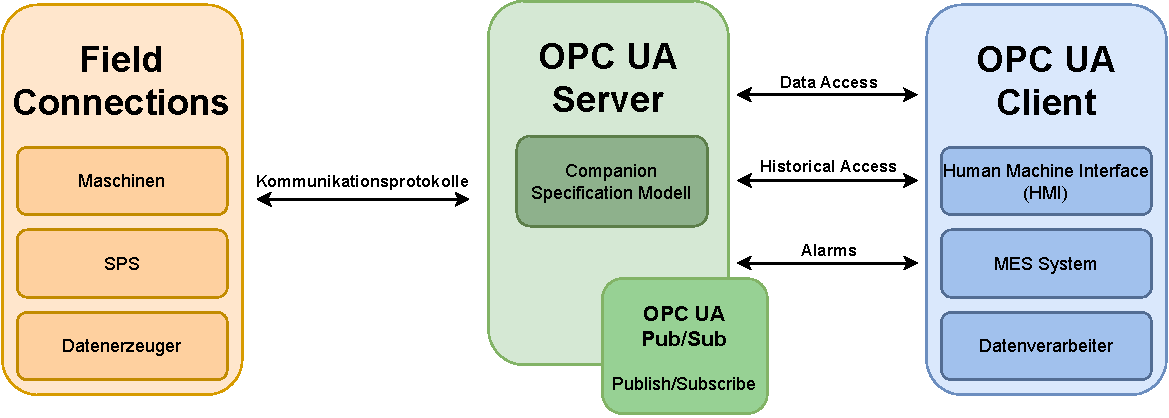
\includegraphics[width=0.9\textwidth]{res/diagramms/OPCUA.pdf}
			\caption{Kommunikationsstruktur OPC UA}
			\label{fig:OPCUA_Structure}
		\end{figure}
		
		In der Automation werden verschiedenste Methoden verwendet, um Endpunkte an eine Anlage anzubinden. In Abbildung \ref{fig:share} sind der Anteil der Verschiedenen Netzwerktypen in der Industrie 2022 veröffentlicht von HMS Networks. Die drei größten Felder sind Fieldbus, Kabellos (Wireless) und Industrielles Ethernet (Industrial Ethernet) wobei letzteres den größte Anteil ausmacht mit 66\%. OPC UA vereint diese Kommunikationsprotokolle in einem Server und so können Clients die Daten über den OPC UA Server auslesen und müssen nicht für jede Maschine ein eigenes Protokoll implementieren. \cite{noauthor_2022_nodate}
		
		Anders Hansson, Chief Marketing Officer von HMS Networks erklärt sich den Wachstum des Industriellen Netzwerkmarktes aufgrund der steigenden nachfrage in der modernen Industrie, nachhaltig, effizient und produktiv zu bleiben und gleichzeitig flexibele und qualitative Fertigung zu ermöglichen. Die Netzwerke zur Kommunikation sind dabei ein Schlüsselfaktor um die genannten Punkte zu erreichen \cite{noauthor_2022_nodate}. Bei einem instgesamten Wachstum der Nutzung dieser Systeme um 8\% zeigen die Entwicklungen in diesen Bereichen eine deutliche Relevanz für die Automatisierung von und Kommunikation mit Maschinen. 
		
		% TODO Kommunikationsprotokolle Analyse Anteile, verwendung AZO
		
		\begin{figure}[H]
			\centering
			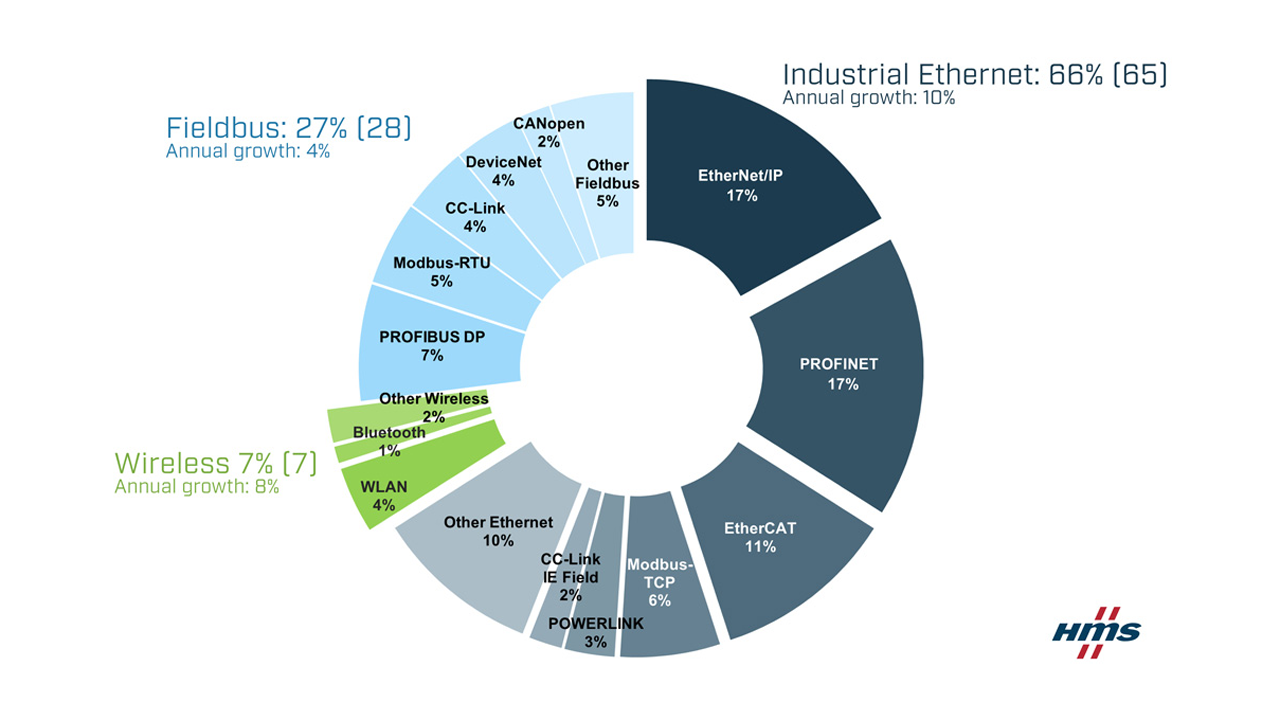
\includegraphics[width=0.9\textwidth]{res/network-shares.png}
			\caption{2022 Industrial network market shares according to HMS Networks \cite{noauthor_2022_nodate}} 
			\label{fig:share}
		\end{figure}
	
		%Nachrichtenaufbau
		OPC UA nutzt einen objektorientierten Ansatz zum Datenaustausch. Dabei werden hierarchische Daten übergeben. Jedes Objekt kann aus Attributen und Methoden bestehen. Die Attribute beinhalten Werte welche gelesen werden können, währen die Methoden vom Client aufgerufen werden können, um der Maschine eine Nachricht zu senden. 
		
		\subsection{Sicherheit}
		
		%Einführung
		Eines der Ziele von OPC UA ist es, eine sichere Verbindung und Kommunikation zu ermöglichen. Die zweite Spezifikation von OPC UA mit dem Titel \glqq Security Modell\grqq definiert die Sicherheit und ist Voraussetzung für die anderen Spezifikationen. Hierin ist festgelegt, welche Sicherheitsmechanismen bei der Nutzung von OPC UA angewendet werden sollen.
		
		% Allgemeines
		Die OPC Foundation beschreibt Unified Architecture mit den Attributen sicher und Firewall freundlich, da OPC UA über den Port 443 kommuniziert, der meist nicht durch Firewalls blockiert wird. OPC UA unterstützt Security auf Transport- und Applikationsebene anhand von selbst entworfenen Protokollen und Erweiterungen von bereits bestehenden Standards. Die Codierung findet auf binärer Ebene statt, wobei die Kommunikation über HTTPS abläuft. Die Authentifizierung von Clients und Servern findet über X509 Zertifikate statt, wobei der Entwickler der UA Anwendung die Anbindung an einen Zertifikatsspeicher selbst übernehmen kann. \cite{noauthor_unified_nodate, noauthor_opc_nodate}
		
		% Authentifizierung/Autorisierung
		Auf Applikationsebene gibt es Sicherheitsmechanismen, welche dir Authentifikation und Autorisierung der Nutzer bearbeiten. Hierbei kommen Passwörtern, Zertifikaten, Webtokens und weiteres zum Einsatz. Außerdem können mit Rechten für Nutzer weitere Einschränkungen auf den Zugriff einzelner Nutzer gelegt werden. Zuzüglich können Aktivitäten von Nutzern und dem System geloggt werden, um die Nachvollziebarkeit zu erhöhen und die Sicherheit des Systems zu stärken. \cite{noauthor_unified_nodate, noauthor_opc_nodate}
		
		%Bundesamt Studie
		Das Bundesamt für Sicherheit in der Informationstechnik führte 2017 eine Sicherheitsanalyse in Kooperation mit TÜV Süd aus und konnte kleine systematischen Fehler in der Sicherheit entdecken. Sie schreiben OPC UA eine hohe Sicherheit zu, wenn die  Mode Sign und security Mode SignAndEncrypt verwendet werden. \cite{damm_opc_2017}
		
		
		%Wenn bei Umati sich etwas ändert, dann dort noch ein Kapitel puschen
	
	\section{\ac{Umati}}
		
		%Einführung
		\ac{Umati} ist eine globale Initiative zur Standardisierung von Schnittstellen zur Kommunikation zwischen Produktionsanlagen. Sie wird vom \ac{VDMA} und dem \ac{VDW} verwaltet, die durch ihre zahlreichen Mitglieder den Standard schnell vorantreiben können. Das Ziel ist es, die Kommunikation zwischen Maschinen möglichst einfach, sicher und einfach zu gestalten. Es soll eine Plug \& Play Umgebung entstehen, in der neue Maschinen in eine Anlage durch bloßes Einstecken ins Kommunikationsnetzwerk integriert werden können. Die \ac{Umati} Initiative entwickelt Standards, welche weltweit zum Einsatz kommen sollen, um eine starke internationale Gemeinschaft um diesen Standard zu erreichen. \cite{noauthor_umati_2023}
		
		%OPC UA in UMATI
		\ac{Umati} baut auf den OPC UA Standards der OPC Foundation auf. OPC UA bildet dabei die Basis und definiert, wie und was kommuniziert werden soll. Es legt fest, was die Rahmenbedingungen für Konnektivität und syntaktische Interoperabilität sind. \cite{noauthor_umati_2023} OPC UA ermöglicht es die semantische Interoperabilität über Companion Spezifications zu versichern. Diese werden auch schon in der Industrie eingesetzt weshalb sich \ac{Umati} die Aufgabe gemacht hat, die verschiedenen Spezifikationen zu vereinheitlichen damit beispielsweise die Identifizierung einer Maschine immer gleich abläuft.
		
		% Automatisierungspyramide
		\ac{Umati} soll vor allem die vertikale und horizontale Integration im Unternehmen erleichtern. In Abbildung \ref{fig:Automatisierungspyramide} ist die Automatisierungspyramide nach Siepmann abgebildet. Je tiefer die Ebene in der Pyramide liegt, desto vielfältiger sind die Systeme dieser Ebene. Während ein Unternehmen nur ein \ac{ERP} System verwendet, kann es zahlreiche SPS und noch mehr Ein- und Ausgabesensoren geben. Diese müssen vertikal integriert werden. Dafür werden Daten von den unteren Ebenen in die Systeme weiter oben zur Verarbeitung überreicht. Bei der horizontalen Integration kommunizieren gleichartige Systeme miteinander. Beispielsweise wenn mehrere SPS Daten austauschen oder Daten Abteilungsübergreifend übergeben werden, wie bei einem Datenfluss von SCM zu CRM System sein. 
		
		\begin{figure}[H]
			\centering
			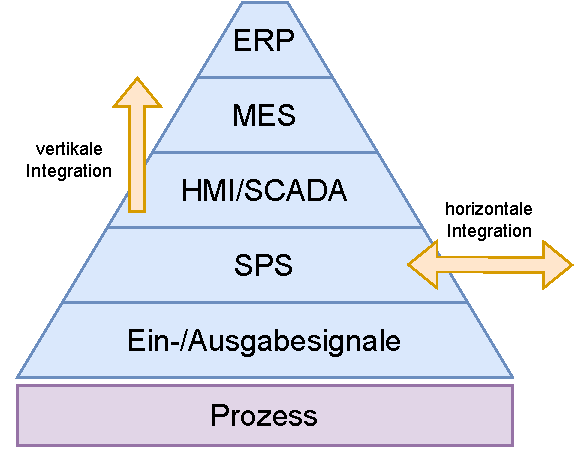
\includegraphics[width=0.8\textwidth]{res/diagramms/Automatisierungspyramide.pdf}
			\caption{Automatisierungspyramide nach Siepmann, \\ Angelehnt an: Folie 8 in \cite{mielebacher_verteilte_2021}} 
			\label{fig:Automatisierungspyramide}
		\end{figure}
		
		\ac{Umati} legt standardisierte Schnittellen fest, mit denen die vertikale und horizontale Integration möglichst einfach umgesetzt wird. Dadurch kann die Wertschöpfung aus Daten kostengünstiger ablaufen und die Analyse, Verarbeitung und Verwertung von Daten, wie es in der Industrie 4.0 üblich ist, besser ablaufen. \ac{Umati} hat bereits Vorführungen auf Messen veranstaltet, welche die Funktionsfähigkeit einer \ac{Umati} Umsetzung demonstrieren. \ac{Umati} standardisiert dabei die Integration von Maschinen, deren Installation und ganze IT Produktionsumgebungen. \cite{noauthor_about_nodate}
		
		% Companion Specifikations
		Die semantische Interoperabilität wurde bereits mit OPC UA über die Companion Spezifikationen erreicht. Allerdings entstehen diese Standards in gesonderten Arbeitsgruppen welche auf die Teilnehmer zugeschnitten sind. Dadurch entstehen viele Spezifikationen in vielen verschiedenen Branchen und Maschinen können nicht mehr ohne Übersetzung kommunizieren. \ac{Umati} versucht diesen Umstand durch das Zusammenfassung dieser Spezifikationen zu beheben. Es sollen Maschinen entstehen, die alle die selbe Sprache sprechen und so einfach in neue IT 
		
		\ac{Umati} selbst besteht aus verschiedenen Modulen, welche alle Standards für verschiedene Bereiche definieren. In Abbildung \ref{fig:OPCUA_for_machinery} sind alle Interfaces abgebildet, welche auf der Base Spezifikation OPC 40001 aufbauen. Dieser wird auch OPC 40001 UA for Machinery genannt und ist für die Anlagenbauindustrie gedacht. \ac{Umati} befindet sich noch in der Entwicklung und ist noch nicht vollständig fertiggestellt, deshalb gibt es Interfaces, welche noch nicht umgesetzt, sondern nur geplant sind. \cite{noauthor_machinery_nodate}
		
		\begin{figure}[H]
			\centering
			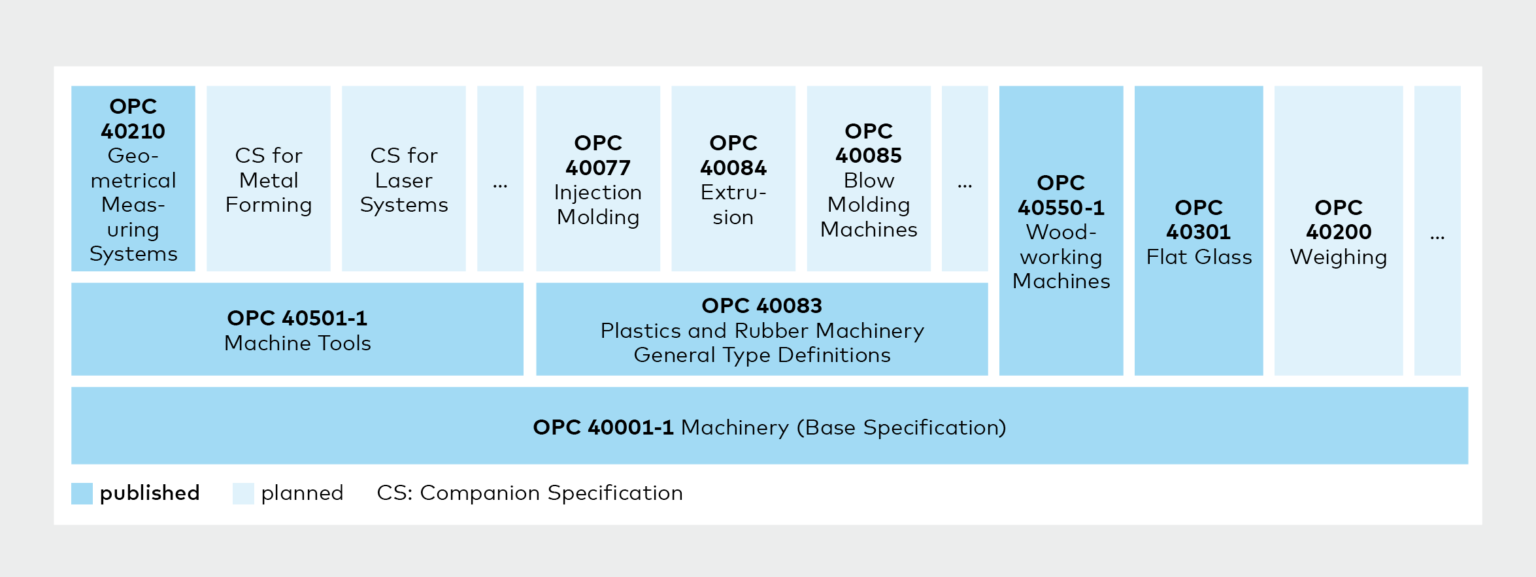
\includegraphics[width=0.9\textwidth]{res/diagramms/OPCUA_for_machinery.png}
			\caption{Interfaces basierend auf OPC UA for Machinery \cite{noauthor_machinery_nodate}} 
			\label{fig:OPCUA_for_machinery}
		\end{figure}
		
		% Kennzahlen, wer nutzt schon, was sind bisherige Meinungen dazu
		
		\subsection{VDMA}
		
		%Allgemin
		\ac{VDMA} ist der größte Industrieverbund in Europa und eines seiner Ziele ist es, \ac{Umati} International zu verbreiten. Der Verband wurde 1892 gegründet und hat seinen Sitz in Frankfurt am Main. Neben der Vertretung der Interessen industrieller Unternehmen in Deutschland und Europa gegenüber der Politik, erarbeitet der VDMA auch Standards und tauscht Know-How zwischen seinen 3.600 Mitgliedsunternehmen aus. \cite{noauthor_verband_nodate} In dem Interessenverband sind Firmen aus den Bereichen Maschinenbau, Anlagenbau und der Zulieferindustrie, welche sich Kompetenzen und Informationen in verschiedensten Themenbereichen von Bildung \& Modernem Arbeiten über Digitalisierung bis zu rechtlichen Feldern teilen. \cite{noauthor_themenubersicht_nodate}
		
		%VDMA Wirken
		Der VDMA wirkt vor allem mit Förderungen in Bereichen, die Innovation bringen. Beispielweise fördert der Verband Technologien in den Bereichen Industrie 4.0, Digitalisierung und nutzt Lobbyarbeit, um seine Mitglieder auch politisch zu unterstützen. Außerdem veranstaltet der VDMA Messen zur Netzwerkbildung und zum Demonstrieren von neusten Technologien seiner Mitglieder. Im Allgemeinen verfolgt der Verband die Stärkung der europäischen Maschinenbaubranche und die Verbesserung der Wettbewerbsfähigkeit auf internationaler Ebene. \cite{noauthor_themenubersicht_nodate}
		
		%AZO
		AZO, der Partner dieser Arbeit, ist auch ein Mitglied des VDMA. Da AZO ein mittelständisches Unternehmen im Anlagenbau ist, setzt sich der VDMA genau für diese Interessen ein und möchte mit \ac{Umati} eine Plug \& Play Umgebung im Anlagenbau ermöglichen. Der VDMA möchte eine erhöhte Interoperabilität zwischen den Maschinen ihrer Mitglieder bewirken und so die Wettbewerbsfähigkeit des europäischen Markts stärken, aber auch in der Standardisierung der internationalen Industrie mitwirken. 
		
		\subsection{OPC UA for Machinery}
		
		\texttt{OPC 40001-1/VDMA 40001-1}, auch OPC UA for Machinery, wurde von VDMA und VDM zusammen mit der OPC Foundation entwickelt. Es ist die fundamentale Spezifikation, auf der andere in diesem Bereich aufbauen sollen. Sie wurde im September 2020 veröffentlicht und seit dem mehrfach aktualisiert worden. Der Standard wird auch in Zukunft erweitert werden, um mehr Use Cases abzudecken. Die neuste Version zum Zeitpunkt des Entwurfs dieser Arbeit ist aus August 2023.
		
		Im Allgemeinen deckt dieser Standard fundamentale Bereiche ab. Es wird definiert, welche Datentypen genutzt werden können, wie deren Syntax ist und wie sie in Attributen abgespeichert werden können. Es werden Objekte und Klassen festgelegt und deren Verhalten und Funktionalität. Darüber hinaus beschreibt die Spezifikation auch, wie ein Client im System die Maschinen an den OPC UA Servern finden kann. 
		
		%TODO: Variablen und Struktur die 40001 definiert erklären, in gut
		OPC for Machinery implementiert keinen festen Typ um als einen Einstiegspunkt für den OPC UA Server. Daher muss auf die Basisspezifikation OPC 40001-1 eine weitere Spezifikation aufgesetzt werden. Im fall dieser Arbeit wird ein Roboter simuliert, weshalb die Spezifikation OPC 40010 Robotics anbietet. Als Mindestanforderung muss Part 1 der Robticsspezifikation imlementiert werden. Dadurch ergibt sich eine anzahl an Variablen, Funktionen und Strukturen, welche in den Simulationsserver implementiert werden und in Kapitel \ref{TOOD: auf anforderungen oder so verweisen}
		
		OPC UA for Machinery definiert, das jede Maschine innerhalb eines Ordners \textit{Machiners} 


	\section{Weitere Technologien}
		\subsection{Docker}
		
		Docker ist eine Open-Source Virtualisierungstechnologie. Ihr primärer nutzen ist das Anbieten, das Entwickeln und Verwalten von Anwendungen auf einem Serverumfeld. Dabei werden alle Services in eigenen Containern verwaltet, was es ermöglicht einzelne Teile einer Anwendung neu zu starten, sie einfach zu skalieren und einzelne Teile zu beenden, ohne das gesamt System zu beenden. Die Container sind auf die Docker-Engine angewiesen, welche zahlreiche Betriebssysteme unterstützt. Ist eine Anwendung containerized, kann sie auf jeder dieser Betriebssysteme auf Basis einer Docker-Engine gestartet werden. \cite{noauthor_install_2023}
		
		Ein Container wird über ein Docker Image gestartet. Ein Image ist der Bauplan einer Anwendung. In einem Docker Compose File können mehrere Container gestartet werden und deren Startparameter festgelegt werden. Zu diesen Parametert gehören benötigte Ports, Umgebungsvariablen für innerhalb des Containers und welche Version des Images verwendet werden soll. Es können auch virtuelle Netzwerke festgelegt werden, welche die Container auch voneinander abgrenzen. 
		
		Docker hat sich im Bereich der Containersysteme durchgesetzt, da es eine zugängliche Schnittstelle zu dieser Art des Servicedeployment bietet. Docker bietet eine einfache Handhabe und Automatisierte Prozesse zum starten und beenden von Services. Docker Hub trug zum Durchbruch der Virtualisierungslösung ebenfalls bei. Dies ist ein Repository im Internet, in dem zahlreiche Images abgelegt werden können. Die Verwendung von Docker hub erfolgt über einen Nativen Docker Befehl, der das Image herunter läd und zur Nutzung bereitstellt. 
		
		Docker ist die grundlegende Technologie für diese Arbeit. Es wird verwendet um die einzelnen Komponenten des Prototypen zu verbinden. Docker eignet sich durch seine einfache Handhabe und die bereits bestehende Expertise im Unternehmen für die Entwicklung des Prototypen. Auch für die Integration in die AZO Infrastruktur bietet sich Docker an, da bereits eine Dockerumgebung für andere Services besteht. 
		
		\subsection{MQTT}
		
		Das \ac{MQTT} ist eine Nachrichtenprotokoll, dass sich durch seine Robusten Eigenschaften vor allem für unzuverlässige Umgebungen eignet. Es ist entwickelt worden um mit Geräten mit hoher Latenz, geringer Bandbreite oder labilem Netzwerk zu kommunizieren. Es eignet sich vor allem für \ac{M2M}-Kommunikation und den \ac{IoT} Bereich, da es besondere Akku und Leistungssparen ist. 
		
		\ac{MQTT} baut auf einer Subscribe and Publish Architektur auf. Ein Eingabegerät, beispielsweise ein Temperatursensor, erhebt seine Daten und reicht sie an einen MQTT Broker weiter, welcher die Daten veröffentlicht (Publish). Möchte ein Client auf die Daten zugreifen, muss er den korrekten \textit{Topic} unter dem die Daten liegen abonnieren und erhält daraufhin alle Änderungen des Datensatzes (Subscribe).
		
		Der\ac{MQTT} Broker übernimmt das Versenden der Daten an alle Clients. Für einen Client sehen die Topics nach einer hierarchischen Struktur aus. Sollte die Verbindung zu einem Client unterbrochen werden, puffert der Broker die Veränderungen an den Daten und sendet diese, wenn der Client wieder verfügbar ist.
		
		%TODO: \subsection{Grafana}
		
\chapter{Methodik}\label{ch:Methodiken}
	% (8 Seiten)
	
	% Forschungsmethodik - Deduktiv??? - Konstruktiv???
	
	\section{Literaturrecherche}
	
	Die Informationen der vorangegangenen Kapitel \ref{ch:Einführung} und \ref{ch:Grundlagen} wurden aus offizieller Literatur der Hersteller entnommen. Zu den Informationen zu OPC UA wurden die offiziellen Spezifikationen und empfohlene Literatur der OPC Foundation verwendet. Dasselbe Vorgehen wurde für die theoretische Vorarbeit von \ac{Umati} genutzt. Die meisten Informationen zum neuen Standard wurden der offiziellen Webseite des VDMA entnommen. Zusätzlich wurden die vom VDMA empfohlenen Literaturen für OPC UA und Umati verwendet. Um theoretische Grundlagen und Konzepterklärungen zu recherchieren, wurden Vorlesungsmaterialien der DHBW Mosbach verwendet.
	
	% Datenerhebung - Literaturrecherche
	% Stichwort recherche
	
	% Über die Hersteller empfolene Literatur
	
	\section{Evaluation}
	
	% Evaluation des Ergebnisses
	
	Das Ergebnis dieser Arbeit ist ein Prototyp zur Demonstration der \ac{Umati} Spezifikation. Dieser Prototyp wurde anhand bestimmter Kriterien bewertet. Diese wurden aus dem Standard ISO 25010 für Softwarequalität entnommen. In Abbildung \ref{fig:ISO25010} sind die Softwarequalitätskriterien strukturiert abgebildet, wie sie im ISO-Standard definiert sind. 
	
	\begin{figure}[H]
		\centering
		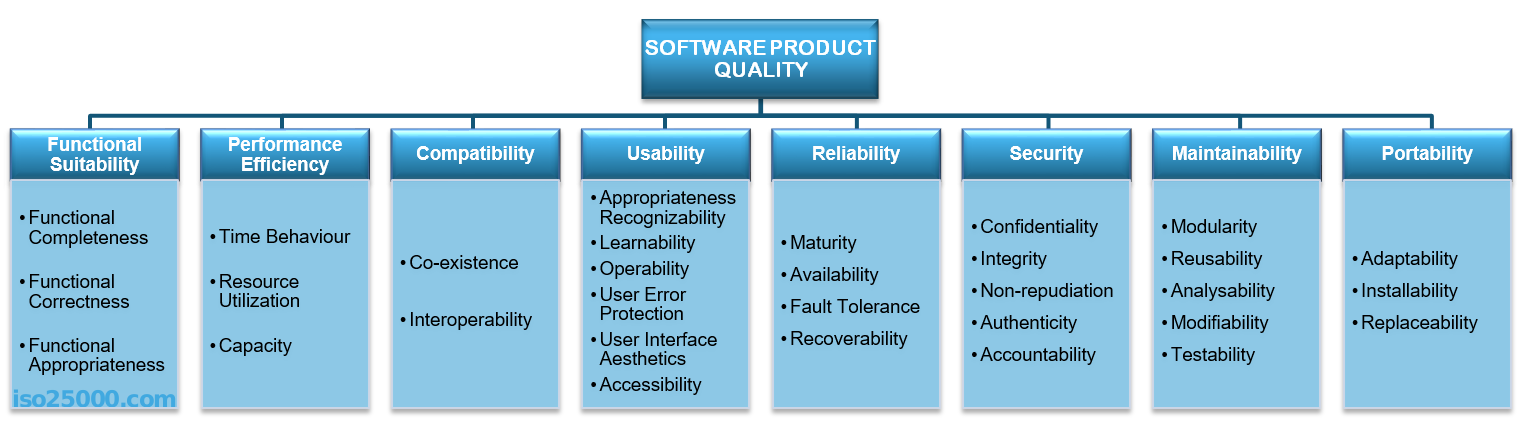
\includegraphics[width=0.9\textwidth]{res/diagramms/iso25010.png}
		\caption{Softwarebewertungskriterien ISO 25010} 
		\label{fig:ISO25010}
	\end{figure}
	
	
	
	Die Punkte \textit{Functional Suitability}, \textit{Performance Efficiency}, \textit{Usability} und \textit{Reliability} sind die Hauptkriterien die für den Messeprototypen besonders wichtig sind. Die anderen Kriterien sind ebenfalls von Wichtigkeit, können jedoch den anderen nachgestellt werden, da der Prototyp nur demonstrativen Nutzen hat. 
	% TODO: Warum???
	% TODO: Quantifizierbare Ziele setzen
	
	Das Demomaterial welches für die Messe ausgelegt werden soll, muss visuell anschaulich sein und die Kernfunktionen von \ac{Umati} präsentieren. Es geht darum das Interesse der Messebesucher zu wecken und genug Informationen für ein allgemeines Bild über die Funktionen und Ziele von \ac{Umati} zu erreichen. 
	
	% TODO: Quantifizierbare Ziele setzen
	
	%TODO: Reflexion
	
	\section{Zeitplanung}
	
	Die Bearbeitungszeit dieser Arbeit beträgt zwölf Wochen, von Montag dem 19.06.2023 bis Montag den 11.09.2023. In Abbildung \ref{fig:Grantt} ist ein Grantt-Diagramm der Zeitplanung abgebildet. In den ersten 4 Wochen sollen die Theoretische Grundlagen und die Analysen der Arbeit abgeschlossen sein, damit die Praxis am 10.07.2023 beginnen kann. Von Woche 5 bis 10 soll die Implementation und Integration des Prototypen stattfinden. Drn gesamte Prozess kann auf gemeinsam 5 Wochen geschätzt werden, wobei eine zusätzliche Woche als Puffer eingeplant wird, sollte es Verzögerungen wie Krankheit oder Bereitstellungsschwierigkeiten geben. Am 21.08.2023 soll die Arbeit abgabebereit sein und für eine Korrekturlesung bereitgestellt werden. Parallel zur Korrekturlesung sollen die Messedokumente und Schulungsunterlagen angefertigt werden. Der letzte Block dient als Puffer für den Abschluss der Arbeit.
	
	\begin{figure}[H]
		\centering
		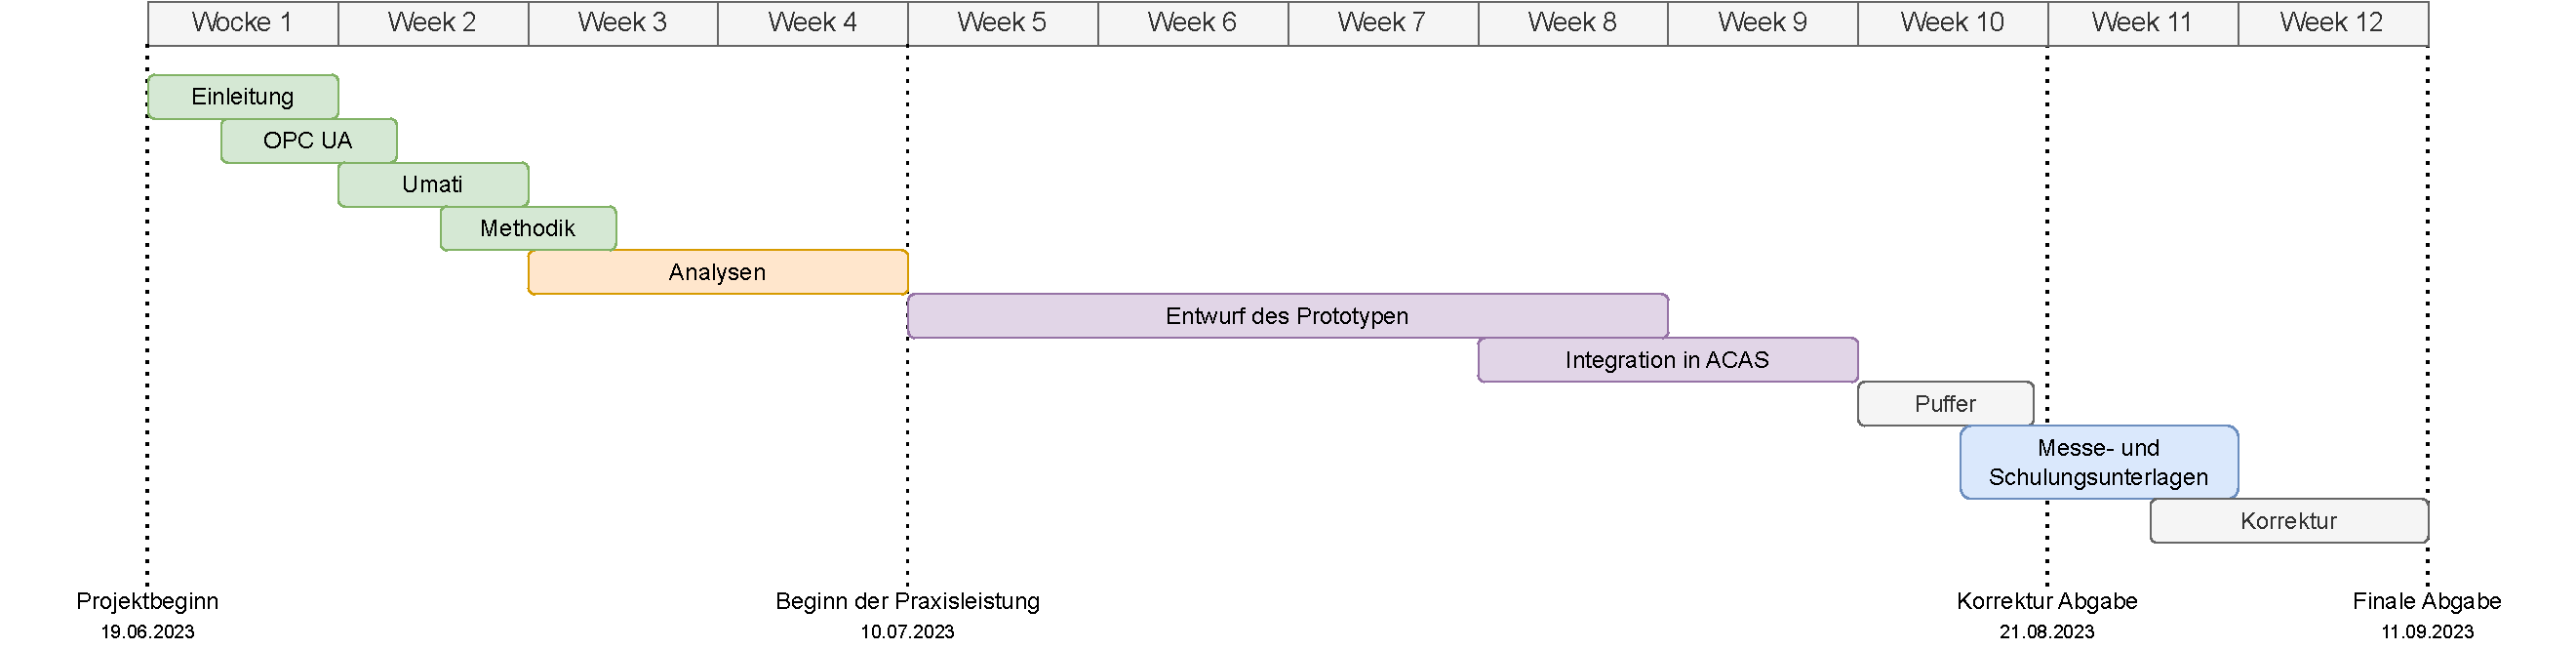
\includegraphics[width=0.9\textwidth]{res/analysen/Grantt-Diagramm.pdf}
		\caption{Grantt-Diagramm zum Projektablauf}
		\label{fig:Grantt}
	\end{figure}
	
	%TODO: Reflexion
	
\chapter{Ergebnisse}\label{ch:Ergebnisse}
	
	% (8 Seiten)
	
	\section{Anforderungsanalyse}
		
		\subsection{Vorgehen}
		%Ziel
		Das Ziel dieses Projekts ist es, die Umsetzbarkeit eines Umatifähigen OPC UA Servers zu demonstrieren. Es sollen Daten von einer Maschine ausgelesen und Angezeigt werden. Es soll eine Struktur entworfen werden, welche den Datenfluss von OPC UA Server an eine Visualisierungsoberfläche ermöglicht.
		
		Zunächst soll der erste Prototyp umgesetzt werden, bei welchem Daten an die offizielle Webseite des VDMAs gesendet werden sollen. Diese Webseite demonstriert, das verschiedenste Hersteller auf einem gemeinsamen Dashboard ihre Maschinen und Anlagen mit Umati integrieren können. AZO möchte eine eigene Maschine dort Anzeigen, welche auf Messen gezeigt werden kann.
		
		Der zweite Prototyp ist eine Verbindung zwischen einem OPC UA Server mit der Umati Implementation und einer internen Visualisierung. Hierbei sollen die Daten aus dem OPC UA Server ausgelesen und so transformiert werden, dass sie auf einem Grafana Dashboard angezeigt werden können. AZO visualisiert bereits bestehende Projekte über Grafana und die Umati Maschinen sollen sich so in die bereits bestehende Infrastruktur eingliedern.
		
		\subsection{Prototyp 1: Umati Web Dashboard}
		
		% Ziel
		Die Daten eines OPC UA Servers soll an das umati Web Dashboard gesendet werden. Die Seite kann unter dem Link \textit{umati.app} erreicht werden. Sie baut auf einem MQTT Broker auf, welcher alle Daten der Teilnehmer abspeichert und an das Dashboard weiter gibt. Der MQTT Broker liegt an der selben Adresse am Port 443 und benötigt Anmeldekriterien für die Veröffentlichung und das Abfragen von Daten.
		
		% Prototyp
		Als Grundlage des ersten Prototypen soll eine Maschine simuliert werden. Es soll keine echte Maschine verwendet werden, da diese eventuell an bestimmten Zeitpunkten ausgeschaltet oder betriebsunfähig sein könnte. Außerdem ist eine laufende Maschine oder Anlage deutlich kostenintensiver als eine serverbasierte Simulation. Die simulierte Maschine soll eine Anlage von AZO darstellen, die auch tatsächlich im Einsatz ist. Als Beispiel wird ein RoLog simuliert, der bei der automatischen Kleinstmengendosierung von Schüttgütern zum Einsatz kommt. In Abbildung \ref{fig:RoLog} ist ein virtualisierter Aufbau der Anlage abgebildet. Der Roboterarm in der Mitte lagert seine Ressourcenbehälter auf den Schränken an der Seite der Anlage, lagert neue Behälter über die Laufbänder an der Hinterseite (Oben-Links) aus oder ein und dosiert in die Ausgabe an der Front (Vorne-Rechts) des Aufbaus. \cite{noauthor_azo_nodate}
		
		\begin{figure}[H]
			\centering
			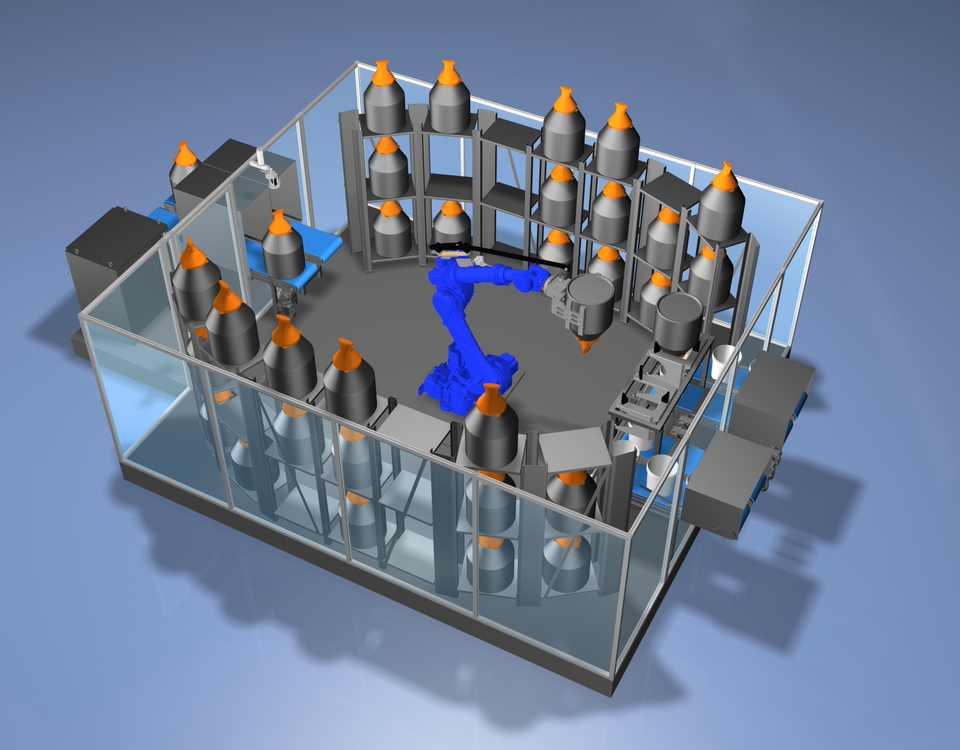
\includegraphics[width=0.7\textwidth]{res/RoLog.png}
			\caption{RoLog von AZO Gmbh \& Co. KG \cite{noauthor_azo_nodate}}
			\label{fig:RoLog}
		\end{figure}
	
		%TODO Text zur Evaluations Kriterien Liste
		
		% Evaluationskriterien
		\begin{itemize}
			\item \textbf{REQ1}: Kommunikation von OPC UA Server zu Client nach Umati Standard
			\item \textbf{REQ2}: Daten auf Umati Web-Dashboard
			\subitem \textbf{REQ2.1}: Visualisierung der Daten, die sich verändern.
			\subitem \textbf{REQ2.2}: Personalisieren aller Daten nach AZO Gmbh.
			\subitem \textbf{REQ2.3}: Anpassen der Location auf der Karte.
			\subitem \textbf{REQ2.3}: Anzeige eines Bild der Maschine.
			\item \textbf{REQ3}: 
		\end{itemize}
		
		\subsection{Prototyp 1: Umati Web Dashboard}
		
		% Ziel
		Die Daten, welche die Simulation der Maschine generiert, sollen an eine Grafana Instanz gesendet werden. Hier soll erneut eine umatifähiger OPC UA Server verwendet werden. Die Daten sollen in der grafischen Oberfläche von Grafana einfach und fasettenreich ausgelesen und Angezeigt werden können. Das Ziel ist es einen Ablauf zu entwerfen, welcher als Ansatzpunkt für zukünftige Projekte verwendet werden kann. 
		
		% Grafana
		Grafan soll dabei in einem Docker-Container laufen. Grafana bietet Nativ die Möglichkeit, unterschiedliche Datenquellen einzubinden. Eine dieser Datenquellen soll verwendet werden. Es soll ein Dashboard entstehen, welches die Daten der Maschine anzeigt und sich live aktualisiert.
		
		%TODO Text zur Evaluations Kriterien Liste
		
		% Evaluierungskriterien
		\begin{itemize}
			\item \textbf{REQ1}: Kommunikation von OPC UA Server zu Client nach Umati Standard
			\item \textbf{REQ2}: Grafan muss in einer Docker Instanz laufen.
			\item \textbf{REQ3}: Dashboard
			\subitem \textbf{REQ3.1}: Visualisierung der Daten, die sich verändern.
			\subitem \textbf{REQ3.2}: Einbinden einer Datenquelle, die Grafana Nativ versteht.
			\item \textbf{REQ4}: 
		\end{itemize}
		
			
		
	\section{Lösungsansatz}
	
		\subsection{Grundlagen}
		% OPC 40001 for Machinery
		Der OPC UA Server muss mehrere Spezifikationen Implementieren. Als Grundlage muss die Identifikation der Maschinen aus der OPC 40001 for Machinery Spezifikation genutzt werden. Der OPC UA Server erstellt dabei einen Namespace, in dem alle Anlagen einem Ordner mit der Bezeichnung \textit{Machines} untergeordnert sind. Jede Komponente und jede Maschine müssen einen Identifikations Ordner Besitzen. Dieser Ordner ermöglicht es, das OPC UA Clients alle Maschinen finden und sie richtig erkennen. 
		
		% OPC 40010 Robotics
		Da die Basisspezifikation jedoch keinen eigenen Einstioegspunkt definiert, muss eine weitere Spezifikation implementiert werden. Diese Arbeit wird die OPC 40010 Robotics - Vertical Integration Spezifikation implementieren. Diese legt fest, welche Komponenten in welcher art und weise vorhanden sein müssen, um ein Maschine im Roboticsumfeld mit Umati zu betrieben. Es muss ein \textit{MotionDeviceSystem}, ein \textit{Robot} und ein \textit{RobotController} existieren. 
		
		% Mandatory Objects
		Der \textit{Robot} implementiert die Axen und Mototren der Maschine und hat ein Attribut mit den Werten der Geschwindigkeit, Beschleunigung und Position. Der \textit{RobotController} verwaltet das \textit{Robot}-Objekt und speichert noch zusätzliche Informationen ab. Beispielsweise welche Software verwendet wird um den Poboter zu steuern und einige Sicherheitsfeatures. Die \textit{MotionDeviceSystem} verwaltet die \textit{RobotController} und stellt die Anlage im ganzen dar.
		
		% Aufbau VM
		Die gesamte Infrastruktur des Projektes wird auf einer VM mit Ubuntu Server 20.04.2 laufen. Auf der VM ist die Docker Engine installiert. Um die Vorgänge auf dem Server besser nachvollziehen zu können ist eine Portainer Instanz als Docker Container installiert. Portainer ist eine grafische Oberfläche die über den Browser erreicht werden kann. Sie ermöglicht den Umgang mit Docker Containern, Images und allem was Docker zu Verfügung stellt sehr einfach. Unter anderem kann eine Console innerhalb der Container gestartet werden, was die Entwicklung extrem vereinfacht. 
		
		\subsection{OPC UA Server}
		
			\subsubsection{OPC UA Server - DataFeed}
				
			Die Softing Industrial Automation GmbH bietet zahlreiche Tools an, um mit OPC UA Servern zu Kommunizieren und auch diese zu entwickeln. Sie bieten unter dem Namen dataFEED OPC Suite Base einProdukt an, welches die Kommunikation mit OPC UA und OPC Classic und die Cloud-Anbindungen übernimmt. Dabei ermöglichen sie die Kommunikation mit führenden Herstellern von Steuerungen wie  Siemens SIMATIC S7, Rockwell ControlLogix, B\&R, Mitsubishi sowie auf Modbus-Steuerungen. \cite{noauthor_datafeed_nodate}
			
			Bei AZO wird diese Suite verwendet, weshalb die Implementierung eines OPC UA Servers mit Umati über dataFEED in frage kam. Allerdings lässt der Baukasten zum Entwurf der OPC UA Server keine Objekte zu, welche notwendig sind, um Umati zu Implementieren.
					
			\subsubsection{Eigenimplementierung}
		
			% Eigenimplementierung in LowCode Plattform NodeRed
			% Muss ich noch rechachieren
					
			Da der Umati Server auf dem Offenen Standard OPC UA aufbaut, kann ein Server auch selbst implementiert werden. Dies hat verschiedene Vor- und Nachteile welche beachtet und auf das Ziel der Implementierung angewandt werden müssen. 
			
			Eigenimplementierungen sind meist Anpassungsfähiger und flexibler, um auf Situationsspezifische Anforderungen zu reagieren. Sie können spezifisch auf den gewünschten Zweck hin optimiert und verbessert werden. Dies kann auch eine einfachere Integration in eine bereits bestehende Umgebung garantieren, da die Anwendung auf diese Umgebung hin angepasst werden kann.
			
			Allerdings kann es auch zu Nachteilen führen. Eigenimplementationen haben ein hohes Risiko auf Fehleranfälligkeiten oder Sicherheitslücken. Bei eingekauften Lösungen profitiert die Anwendung im Normalfall von Erfahrungswerten des Breitstellers und dem Umstand, dass diese Lösung sich bereits am Markt behaupten musste. Die Fehlende Erfahrung kann auch zu einem Programm führen, welches kaum optimiert und komplex ist, was die Wartbarkeit und Nutzerfreundlichkeit vermindert. Soll die Lösung zu kommerziellen Zwecken eingesetzt werden oder hat hohe Anforderungen an Sicherheit, Zugverlässlichkeit und Robustheit sollte auf eine Eigenimplementation verzichtet werden.
			
			Trotz der Nachteile sollte die Umsetzung einer Eigenimplementierung, vor allem zu Demonstrationszwecken, in Betracht gezogen werden. Hierbei gibt es Low-Code und High-Code Ansätze. Bei High-Code Implementierungen wird die Funktionalität in Code hergestellt. Beispielsweise kann ein OPC UA Server nur anhand von Python oder C\# Frameworks implementiert werden. Low-Code Ansätze bedienen sich dabei einem Visuellen Programmierstil. Die Programierung findet über IDEs statt, welche mehr auf Bausteinartige Programmierung setzen. Beispiele für solche Umgebungen sind NodeRed oder Microsoft Power Apps. 
			
			\paragraph{Implementierung mit C\#}
			Die OPC Foundation stellt ein Framework für die Entwicklung von OPC Servern auf C\# Basis zu Verfügung. Die OPC UA.NET Standard Bibliothek ermöglicht die Entwicklung von OPC Servern und Clients. Eine Eigenimplementierung mit diesem Framework würde einen sehr individualisierbaren und flexiblen Server ergeben, welcher den RoLog in seiner exakten Funktion darstellen könnte. Allerdings ist die Implementierung sehr zeitintensiv und benötigt Expertiese auf dem Bereich. \cite{noauthor_opc_nodate-1}
			
			Um eine einwandfreie Simulation eines RoLogs als Basis der Prototypen zu verwenden, sollte diese Implementierung in Betracht gezogen werden. Allerdings ist diese Form um einen ersten \ac{PoC} für Umati zu entwerfen zu aufwendig.
			
			% zu zeitintensiv aber hoch individualisierbar
			% Sollte auch das Ziel sein, vorallem wenn die Simulation richtig gut werden soll
			
			\paragraph{Implementierung in einer SPS}
			Die Implementierung einer OPC UA Schnittstelle kann auch direkt auf einer SPS durchgeführt werden. Siemens SPS stellen einen integrierten OPC UA Server zu Verfügung welcher direkt an der Anlage laufen kann. Es gibt auch die Möglichkeit, Maschinen zu Simulieren und mit kleinen Programmen deren Verhalten zu bestimmen. Der Server der SIMATIC S7 SPS von Simens kann Objekte und Klassenstrukturen darstellen. \cite{noauthor_tia_2019}
			
			Die Entwicklung eines solchen Servers ist sehr Zeitaufwendig und benötigt Expertise im entwickeln von OPC UA Servern auf SPS. Es ist denkbar Maschinen die Umatifähig sein sollen, auf dieser Ebene als OPC UA Server zu entwickeln, allerdings für eine Demonstration von Umati zu Umfangreich.
			
			\subsubsection{Vorgefertigte OPC UA Server mit Umati}
			
			
			
	
	\section{Marktanalyse}
		
		% Lösungen vom VDMA alle vorstellen
		% 
		
	\section{Wirtschaftlichkeit und Projektanalyse}
	
		\subsection{Kostenplanung}
		
		\subsection{Fallbeispiel}
			% Beispielswiese an Fallbeispiel -> Durchschnittliche AZO Straße
			% -> Probleme bei Schnittstellen integrierung.
	
\chapter{Implementierung}\label{ch:Implementierung}
	
	\section{Veröffentlichung von Daten auf dem \ac{Umati} Web-Dashboard}\label{ch:Implementierung-Web}
		
		\subsection{Struktur}
		
		Das Ziel ist eine AZO Maschine auf der \ac{Umati} Demonstrationsseite (https://umati.app) anzuzeigen. In Abbildung \ref{fig:uamti.app} wird die Struktur des Datenaustausches mit der \ac{Umati} Webseite bildlich dargestellt. Die Daten entstehen in der Simulation des RoLogs, der AZO Maschine. Dieser stellt einen Roboter dar, dessen OPC UA Server die Robotics Spezifikation implementieren soll (OPC 40010). \ac{Umati} empfängt Daten über einen MQTT Server und synchronisiert diese Daten dann mit dem umati.app Dashboard. Um aus dem OPC UA Server die Daten an den in der Cloud befindlichen MQTT Server zu senden, kann ein vorgefertigter Dockercontainer der VDMA verwendet werden, um den Transport zu übernehmen. Der Datenbroker kann auf dem \ac{Umati} Github Repository gefunden werden.
		
		Andere Firmen können ihre Daten über den selben Prozess auf das \ac{Umati} Dashboard laden. So entsteht eine Demonstration das eine Oberfläche die Möglichkeit besitzt, Maschinendaten aus verschiedensten Quellen un Herstellern integrieren kann. 
		
		Sind die Daten auf dem \ac{Umati} Server können sie anhand der von VDMA gesendeten Anmeldedaten über einen MQTT Client gelesen werden und daraufhin in das lokale MES System integriert werden.
		
		%TODO: Auf interesanteste Repositories eingehen
		
		\subsection{RoLog OPC UA Server}
		
		\subsection{Dashboard OPC UA Client}
		
		\subsection{MQTT Server und Web-Dashboard}
	
	
	\section{Implementierung eines Prototyps}\label{ch:Implementierung-Intern}
	
		\subsection{Struktur}
		
		% VDMA Repositories
		Der VDMA und VDA, die Operatoren von \ac{Umati}, haben eine Kollektion von Repositories auf Github, auf welchen multiple Implementationsmöglichkeiten eines \ac{Umati} Servers dargestellt sind. \cite{noauthor_github_nodate} All diese Projekte sind bereits auf Vollständigkeit geprüft und garantieren so die volle umsetzen der \ac{Umati}-Standards, oder zumindest einer angegebenen \ac{Umati} Spezifikation. Beispielsweise kann ein Sample-Server verwendet werden, um einen \ac{Umati}-Server aufzusetzen, der pseudo-zufällige Werte generiert und diese zur Abfrageung bereit stellt. Dieses Repository implementiert zum Zeitpunkt der Abfrage im August 2023 die Spezifikationen \textit{Machine Tool}, \textit{Woodworking}, \textit{Geometrical Measurement Systems} und \textit{Additive Manufacturing} und simuliert Maschinen, welche die notwendigen und optionalen Variablen implementieren, die sie festlegen.
		
		% Relevanz
		Dieses Verzeichnis beinhaltet auch weitere Implementierungen von Demonstrationsservern in verschiedenen Programmiersprachen umd mit abweichenden Companionspezifikationen von \ac{Umati}. Für dieses Projekt sind vor allem der Sample-Server-node-opcua und Dashboard-OPCUA-Client von relevanz. 
		
		% Die zwei Repositories
		Der Sample Server stellt mit Standardeinstellungen einen OPC UA Server zur verfügung, der mehrere Maschinen im Hintergurnd nach den verschiedenen Spezifikationen simuliert. Es existiert Beispielsweise ein Simulation, die einen Roboter darstellt, der seine die Geschwindigkeit und die Position des Arms mit pseudo-zufälligen Werten beschreibt und in kurzen Abständen ändert. Das Dashboard fungiert als übersetzer zwischen dem MQTT Broker welcher umati.app nutzt und dem zuvor OPC UA Server, welcher die Maschine simuliert.
		
		% umati.app
		Die Daten der simulierten Maschine soll auf die umati.app des VDMA gestreamt werden und dort genau wie die bereits vorhandenen Maschinen angezeigt werden. Dafür müssen die daten in einen \ac{MQTT} Server gespeicher werden, welcher dann im Hintergrund die Kommunikation mit der Webanwendung übernimmt. 
		
		% Struktur des Datenfluss
		In Abbildung \ref{fig:umati.app} wird der Datenfluss visuall abgebildet. Die Daten entstehen in der Simulation des RoLogs, welcher einen OPC UA Server nutzt, um Seine Daten zu versenden. Dank der Implementierung der \ac{Umati} Spezifikation kann der OPC UA Client des VDMA den  RoLog erkennen und dessen Daten an den \ac{MQTT} Server der umati.app weiterleiten. Dort werden die Daten so verarbeitet, dass sie auf dem Dashboard im Internet angezeigt werden können. Andere Teilnehmer an dem Projekt können über den selben Prozess ihre Daten an den \ac{MQTT} Server senden, und so entsteht Dashboard, mit mehreren Maschinen von verschiedensten Anbietern.
		
		% Retrieve
		Der MQTT Server der umati.app kann auch abonniert werden, um die Daten in ein eigenes Projekt zu überführen. Alternativ, um den Weg über das Internet zu vermeiden kann der OPC UA Client des VDMA auch umkonfiguriert werden, um auf einen lokalen \ac{MQTT} Server zu senden. 
		
		\begin{figure}[H]
			\centering
			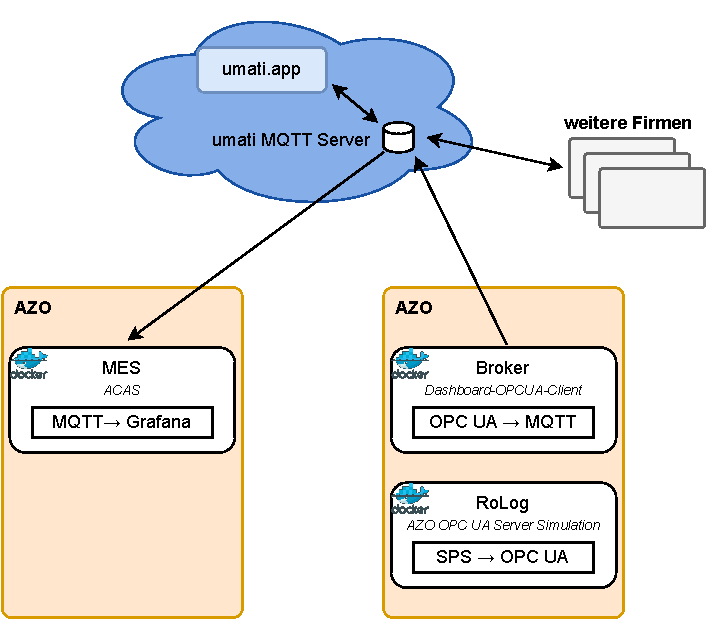
\includegraphics[width=0.9\textwidth]{res/umatiAppStruktur.pdf}
			\caption{Datenfluss und Struktur des Prototypen}
			\label{fig:umati.app}
		\end{figure}
		
		 
		\subsection{Sicherheit}
		
		Die Demonstration über die \ac{Umati} Webapplikation dient nur Messezwecken und sollte nicht für die Produktion verwendet werden. Der Aufbau einer \ac{Umati} Umgebung sollte in einem lokalen Umfeld passieren, mit den maximalen Authentifizierungsmöglichkeiten die \ac{Umati} zulässt. %TODO: Das ist doch nix
		
		\subsection{OPC UA Server}
			
		Der OPC UA Server besteht aus zwei Komponenten. Der Simulation des Roboters und die Implementierung der \ac{Umati} Spezifikation OPC 40010 - Robotics. Um den OPC UA Server zu Verfügung zu stellen wurden mehrere Ansätze verwendet die in diesem Kapitel diskutiert werden. Die für diese Arbeit am besten geeignetste Lösung ist die Verwendung eines Sample Server Forks des \ac{Umati} Repositories der mit den Daten eines RoLogs oder zu simulierenden Maschine beschrieben wird. 
		
			\subsubsection{dataFeed Server}
			
			DataFeed wurde von Softing Industrial Automation GmbH entwickelt welche ein „All-in-One“-Datenintegrationslösung für die OPC UA-Kommunikation anbieten.
			
			Mit dem dataFeed Tool können einfache OPC UA Server implementiert werden, welche Variablen und einzelne Attribute übermitteln können. \ac{Umati} verlangt eine  Objektbasierte Strukturierung der Daten, welche anhand der limitierten von dataFeed nicht umsetzbar ist.
			
			\subsubsection{Eigenimplementierung}
			
			
			\subsubsection{Sample Server - \ac{Umati}}			
			
			
			Die schnellste und robusteste Lösung für den Upload der Daten auf die \ac{Umati}-App ist es, den von Andreas Heine entwickelten Sample-Server-Node-opcua aus dem \ac{Umati} Verzeichnis auf Github zu verwenden. Diese erstellt eine Simulation von mehreren Maschinen und deren OPC UA Servern, welche alle eine andere Schnittsteller der \ac{Umati} Spezifikationen anbieten. Das Projekt umfasst die Spezifikationen OPC 40010 UA for Robotics, OPC 40550 UA for Woodworking, OPC 40501 UA for Machine Tools und noch weitere auf einzelne Herrsteller spezialisierte Schnittstellen. Der Sample Server kann in einem Dockercontainer gestartet werden kann daraufhin über den Port 4840 als OPC UA Server angesprochen werden. Um den Container mit einer VDMA Sample Maschine zu starten kann folgender Docker Befehl ausgeführt werden:
			
			\begin{lstlisting}[numbers=none, language=bash, frame=single]
docker run -it -p 4840:4840 -e PORT=4840 -e IP=127.0.0.1 --name sampleserver-node-opcua ghcr.io/andreasheine/sampleserver-node-opcua:main
			\end{lstlisting}
			
			Die Werte und variablen die die Maschine Anzeigt, wie beispielsweise Name, Location und Hersteller können in einer XML-Datei angepasst werden. Unter dem Ordner \textit{models} können für jede Art der Maschine Werte geändert werden. Um diese dann auch verwenden zu können, wurde ein Ford des Reposetories von Andreas Heine erstellt und die Werte in den XML FIles verändert. Um den Container einfach starten zu können wurde folgendes Docker Compose File erstellt:
			
			\lstinputlisting[frame=single]{res/code/compose-rolog.yaml}
			
			Dieses Docker Compose File startet einen Container mit dem Namen \textit{opcua-rolog} aus dem Ordner in dem es Abgespeichert ist. Diese Datei sollte im Selben Ordner wie das Dockerfile des Forks für den Sample Server liegen. Es verbindet den Port 4840 des Hostsystems mit dem Port 4840 des Containers. Wird nun eine Anfrage an den Port des Hostsystems gesendet, reicht dieser sie an den Port des Containers weiter. Dieser Port kann auch eine anderer sein, sollte 4840 bereits belegt sein (Beispiel: "4841:4840" um den Port 4841 des Hostsystems zu verwenden). Der Container kann mit einem Docker Compose Befehl gestartet werden. 
			
			\begin{lstlisting}[numbers=none, language=bash, frame=single]
docker-compose -f docker-compose.yaml up
			\end{lstlisting}
			
			
			%TODO: Server Erklären
			
		\subsection{OPC UA Client}
		
		Der OPC UA Client hat die Aufgabe die Daten des Servers zu erfragen und sie an den MQTT Broker weiter zu geben. Der Client muss die \ac{Umati} Spezifikationen lesen können und die Identifikation der Maschinen durchführen.
		
			\subsubsection{\ac{Umati} Dashboard OPC UA Client}
			
			Für den Upload der Daten auf die umati.app Webseite, ist der vorgefertigte Client des VDMAs gedacht. Dieser verwendet eine Konfigurationsdatei um zu definieren, welche Spezifikationen er implementieren muss, welchen OPC UA Server er ansprechen kann und wo der MQTT Server liegt, welcher verwendet werden soll. In Anhang I ist die Konfigurationsdatei aufgeführt. Sie beinhaltet alle Wichtigen Informationen um einen Server zu starten, der die Robotics Spezifikation implementieren soll. Von besonderer Wichtigkeit sind die beiden Felder \textit{OpcUa} und \textit{Mqtt}. Die Variable \textit{OpcUa} zeigt auf den OPC UA Server, welcher als Dockercontainer gestartet wurde. Es können auch Authentifizierungsmöglichkeiten von \ac{Umati} verwendet werden, wobei die Anmeldedaten und die Authentifizierungsart eingetragen werden müssen.
			
			\lstinputlisting[firstline=37,lastline=42,frame=single]{res/code/config.json}
			
			In der Konfigurationsdatei muss ein MQTT Broker angegeben werden, an den die Daten gesendet werden sollen. Zum Testen der \ac{Umati} Schnittstelle und des Aufbaus der Container kann hier zunächst ein lokaler Server eingetragen werden. Funktioniert die gesamte Übertragung der Daten, können die Informationen mit den Anmeldedaten des \ac{Umati} MQTT Brokers ausgetauscht werden. Im folgenden Codebeispiel sind die Daten für die Verbindung mit dem \ac{Umati} MQTT Broker angegeben.
			
			\lstinputlisting[firstline=43,lastline=51,frame=single]{res/code/config.json}
			
			Der MQTT Broker sitzt unter der adresse \textit{umati.app} an dem Port \textit{443} und nutzt einen Web Sockert zur Kommunikation. Die Anmeldedaten müssen beim VDMA angefragt werden und die \ac{MoU} unterzeichnet werden.
			
			\subsubsection{Eigenimplementation}
			
			Eigenimplementierungen eines OPC UA Client ist sehr Zeit- und Resasourcenintensiv. Die Daten können jedoch auf jede erwünschte weise ausgegeben werden. Allerdings wiegt hier der Nachteil schwerer, da das Projekt Zeitlich sehr strikt begrenzt ist. Da es bereits entwickelte Möglichkeiten für einen OPC UA Client des VDMAs gibt, lohnt sich die Eigenimplementierung nicht. Die selben Prinzipien können auch auf eine Implementierung in Node Red angewandt werden.
			
		
		\subsection{MQTT Broker}
			% MQTT Broker der Daten speichert und veröffentlicht
			
			% Probleme und Lösungen
		
		\subsection{Integration in bestehende Infrastruktur}
			% Integration in Unternehmensstruktur
			

	
	
	\chapter{Diskussion und Fazit}\label{ch:Diskussion_Fazit}
	
		% (2-5 Seiten)	
	
		% Disskussion -> Subjektive Bewertung der Spezifikation UMATI, ... Literaturpunkte meine Meinung, Sinnvoll Einzusetzen
	
	\printbibliography
	\frontmatter
	
	\pagebreak
	\section*{Anhang I: configuration.json} \label{Anhang1} %TODO: Überschrift aus Inhalt raus
	\lstinputlisting{res/code/config.json}
	\pagebreak

\end{document}
